%! Author = gramic
%! Date = 21.04.24

% Preamble
\clearpage
\KOMAoptions{paper=A4,paper=portrait,pagesize}
\recalctypearea
\begin{flushleft}
%    \clearpage
%    \KOMAoptions{paper=A4,paper=portrait,pagesize}
%    \recalctypearea
    \subsection{Maintenance - YugabyteDB}
    \label{subsec:maintenance_yugabytedb}
    Das Projekt hat eine sehr hohe Anzahl an aktiven Issues, wobei viele neue dazugekommen sind:
    \begin{figure}[H]
        \centering
        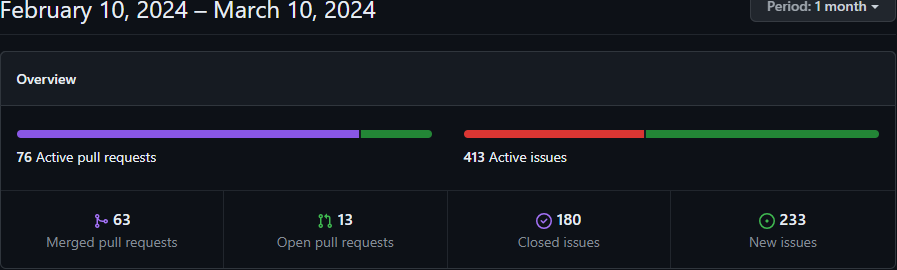
\includegraphics[width=0.75\linewidth]{source/implementation/evaluation/postgresql_ha_solutions/insights/yugabytedb/pulse_yugabyte_yugabyte-db}
        \caption{YugabyteDB - Pulse}
        \label{fig:pulse_yugabyte_yugabyte-db}
    \end{figure}

    Die Code Frequency kann nicht ausgegeben werden, es gab zu viele Commits:
    \begin{figure}[H]
        \centering
        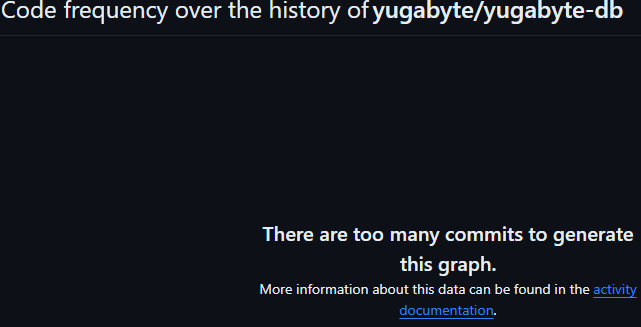
\includegraphics[width=0.75\linewidth]{source/implementation/evaluation/postgresql_ha_solutions/insights/yugabytedb/code_frequency_yugabyte_yugabyte-db}
        \caption{YugabyteDB - Code Frequency}
        \label{fig:code_frequency_yugabyte_yugabyte-db}
    \end{figure}

    Das Projekt hält nur die wichtigsten Community Standards ein:
    \begin{figure}[H]
        \centering
        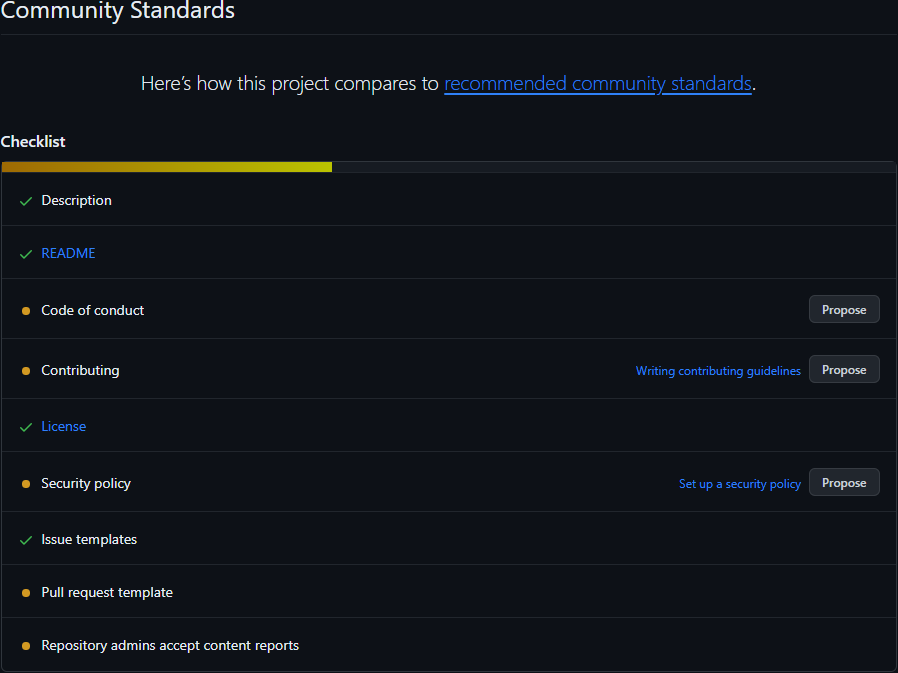
\includegraphics[width=0.75\linewidth]{source/implementation/evaluation/postgresql_ha_solutions/insights/yugabytedb/community Standards}
        \caption{YugabyteDB - Community Standards}
        \label{fig:community Standards_yugabyte-db}
    \end{figure}

    Es werden immer wieder Commits abgesetzt, allerdings sind diese nicht weiter aufgeteilt in Commits, Additions und Deletations:
    \begin{figure}[H]
        \centering
        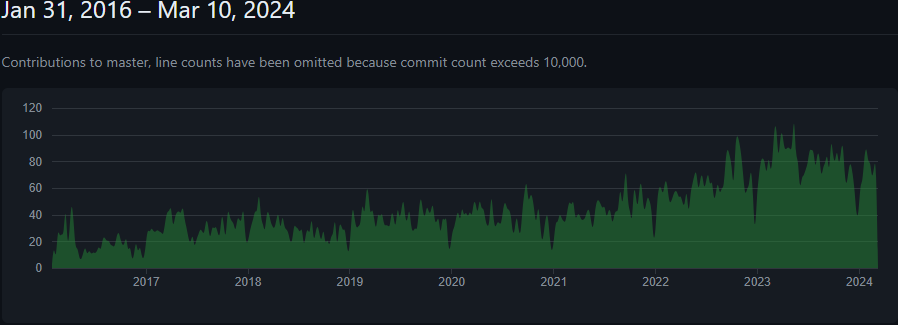
\includegraphics[width=0.75\linewidth]{source/implementation/evaluation/postgresql_ha_solutions/insights/yugabytedb/contributors_to_yugabyte_yugabyte-db}
        \caption{YugabyteDB - Contributors}
        \label{fig:contributors_to_yugabyte_yugabyte-db}
    \end{figure}
\end{flushleft}
\clearpage
\KOMAoptions{paper=A4,paper=portrait,pagesize}
\recalctypearea
\begin{flushleft}
    Die Commits wiederum werden regelmässig ausgeführt, es wird scheinbar in kurzen Sprints gearbeitet:
    \begin{figure}[H]
        \centering
        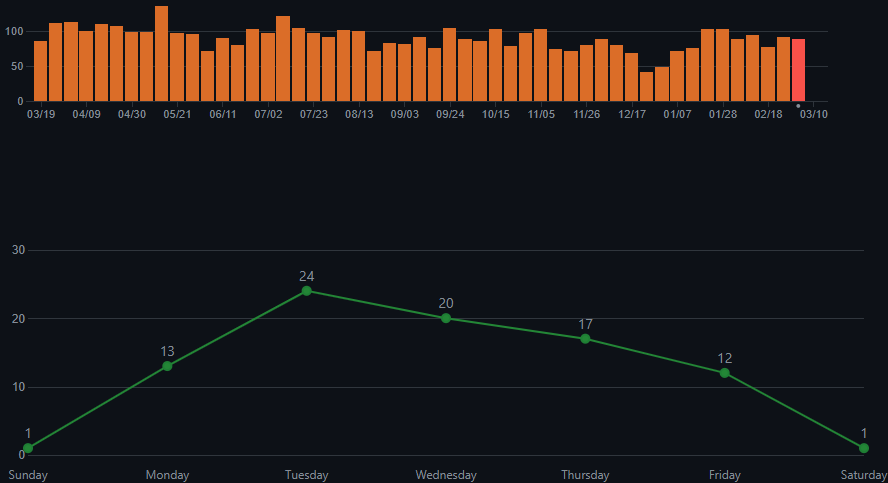
\includegraphics[width=0.75\linewidth]{source/implementation/evaluation/postgresql_ha_solutions/insights/yugabytedb/commit_activity_yugabyte_yugabyte-db}
        \caption{YugabyteDB - Commit Activity}
        \label{fig:commit_activity_yugabyte_yugabyte-db}
    \end{figure}
    YugabyteDB ist der Maintainer seines Produkts.\\
    Es gibt keine anderen grossen Contributors:
     \begin{figure}[H]
        \centering
        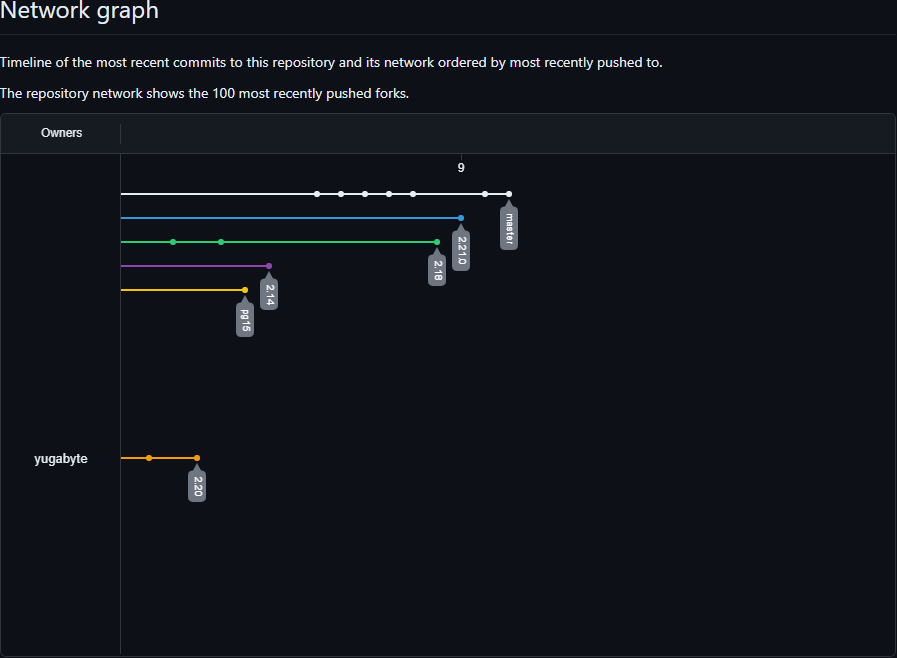
\includegraphics[width=0.75\linewidth]{source/implementation/evaluation/postgresql_ha_solutions/insights/yugabytedb/network_graph_yugabyte_yugabyte-db}
        \caption{YugabyteDB - Network Graph}
        \label{fig:network_graph_yugabyte_yugabyte-db}
    \end{figure}
\end{flushleft}